\chapter{Running Examples}

This chapter provides a detailed walkthrough of our application's functionalities through a series of screenshots. Each screenshot is accompanied by an explanation of the feature it represents, illustrating the user experience from registration to interaction with the various components of the platform.

When a user first visits the site, they are presented with a search bar, as depicted in Figure \ref{fig:searchbar}. This feature allows unregistered users to search for places by name or postcode. Upon entering a search query, users are redirected to a detailed place page, which includes a map and comprehensive information about the location.

\begin{figure}[H]
    \centering
    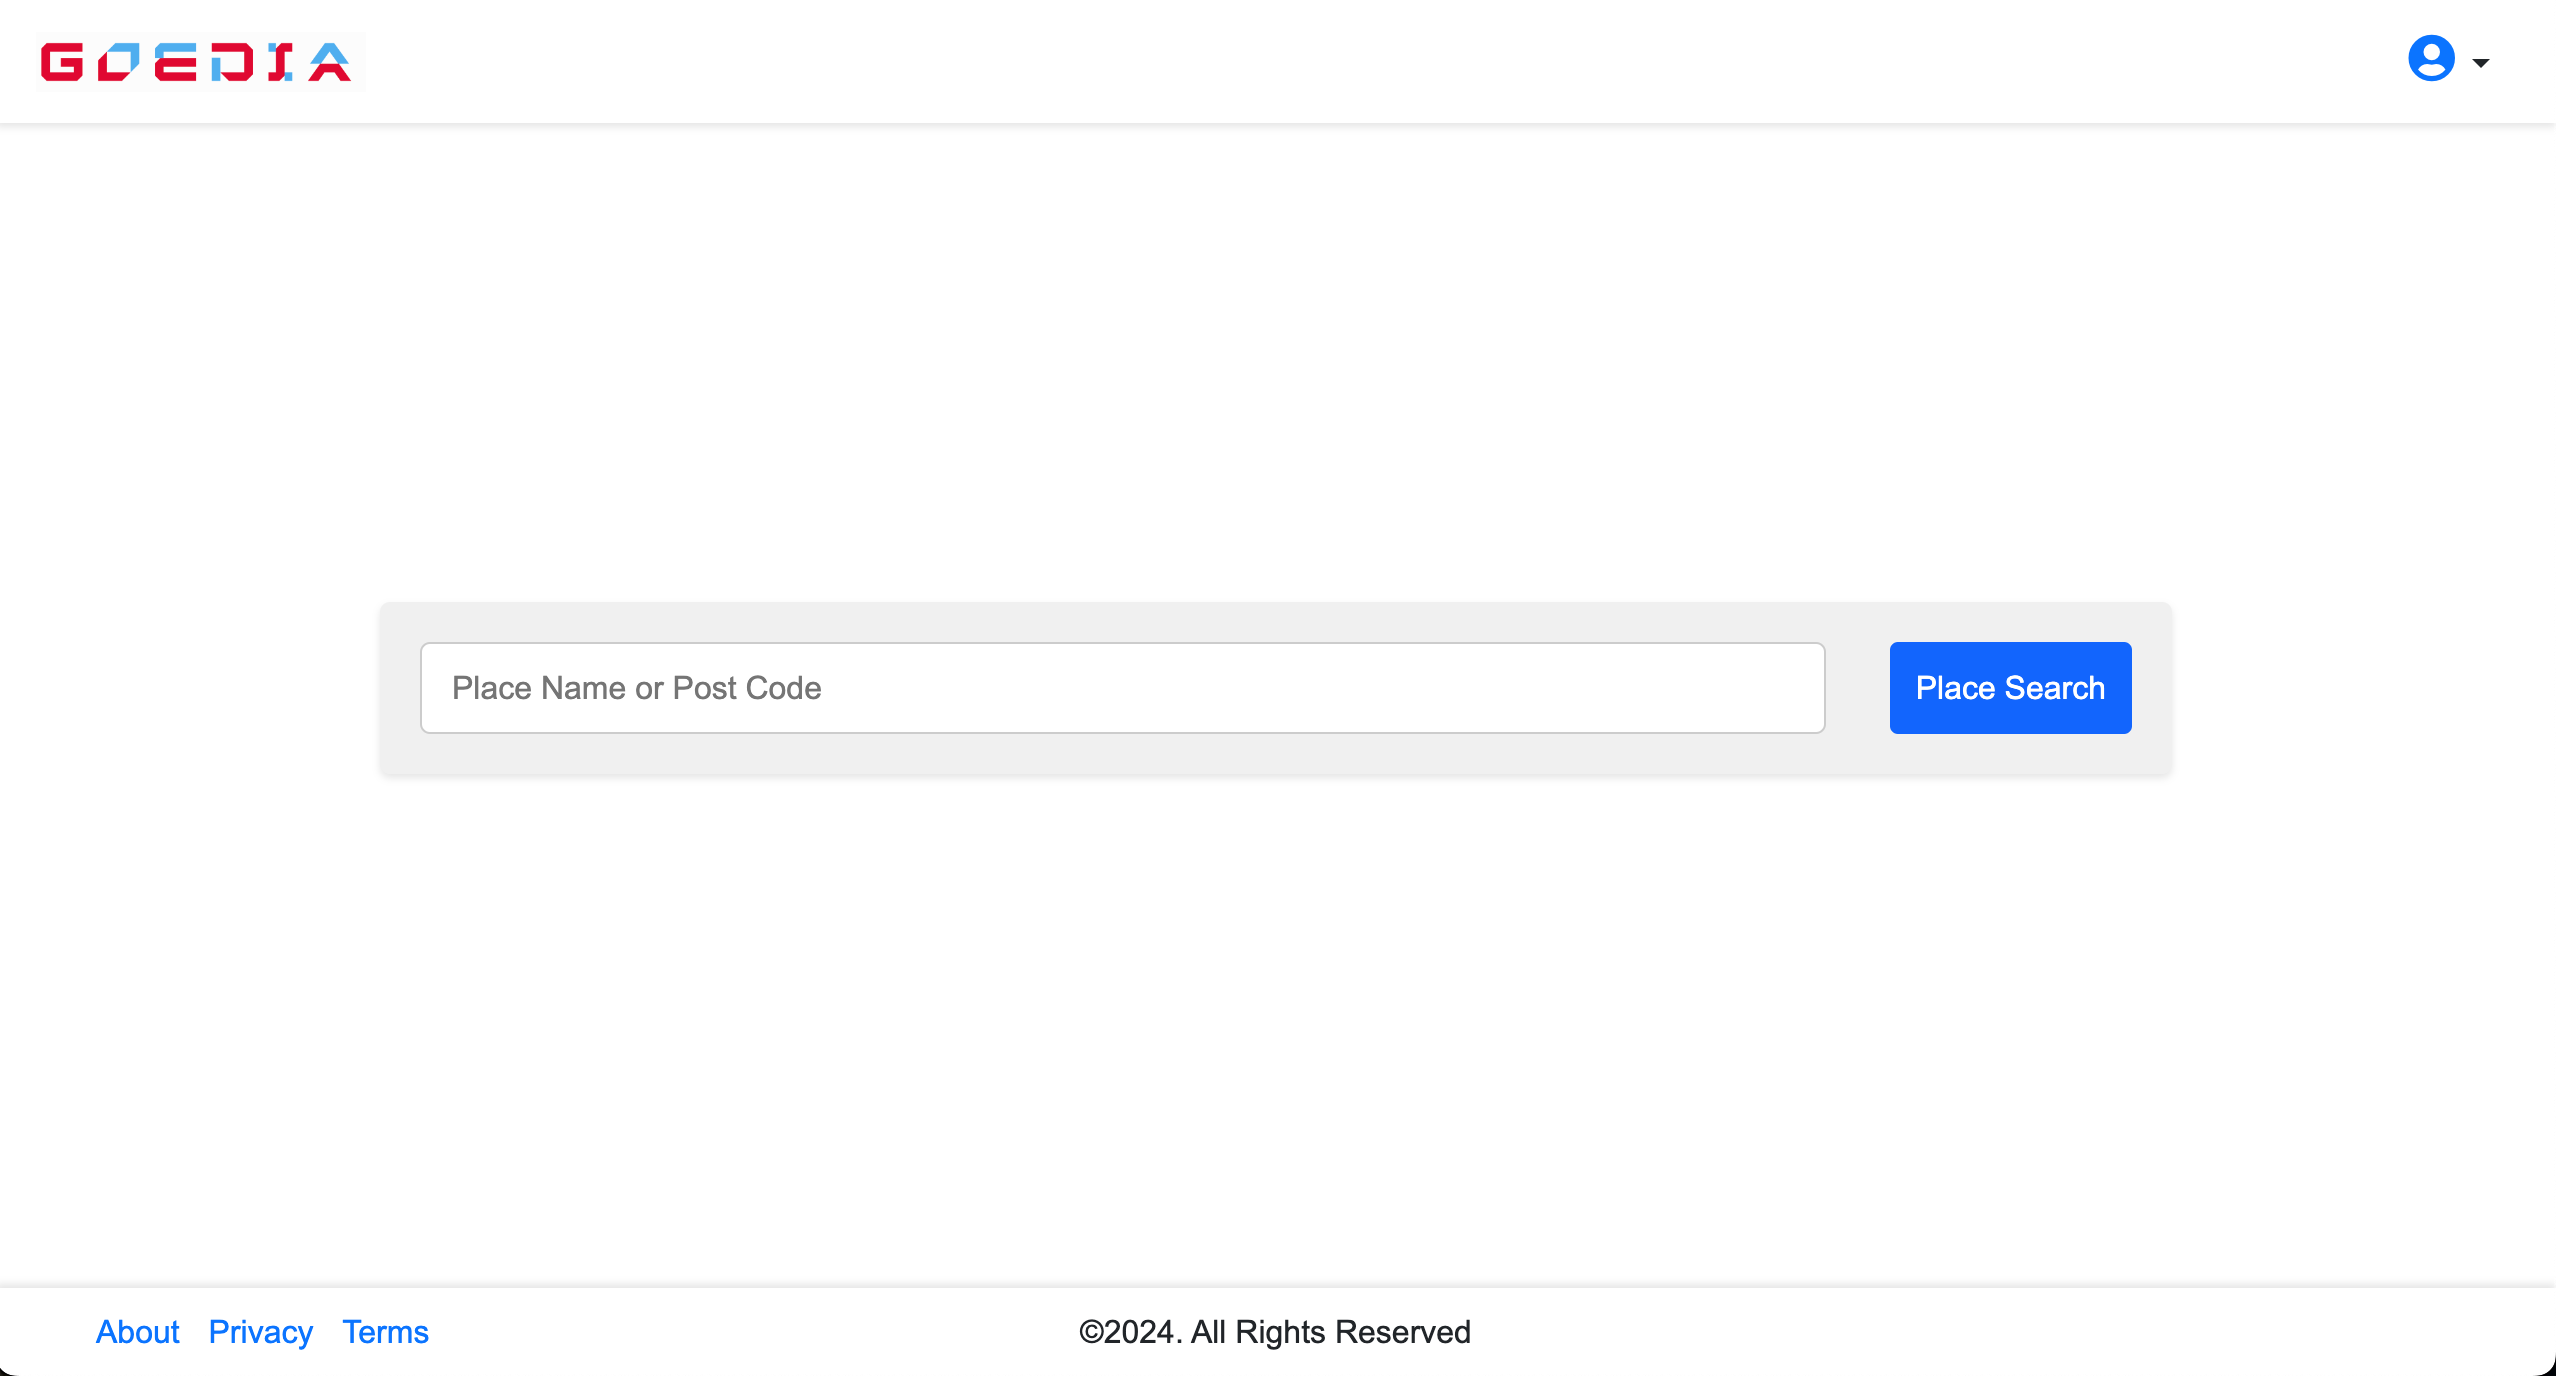
\includegraphics[width=\textwidth]{searchbar.png}
    \caption{Search Bar for Unregistered Users}
    \label{fig:searchbar}
\end{figure}

If the user chooses to register, they can click on the "Register" button at the top right of the screen, which takes them to the registration form. The registration form, depicted in Figure \ref{fig:signup}, prompts the user to provide essential details such as their full name, email address, password, and date of birth. This form is straightforward and user-friendly, ensuring a smooth onboarding process for new users.

\begin{figure}[H]
    \centering
    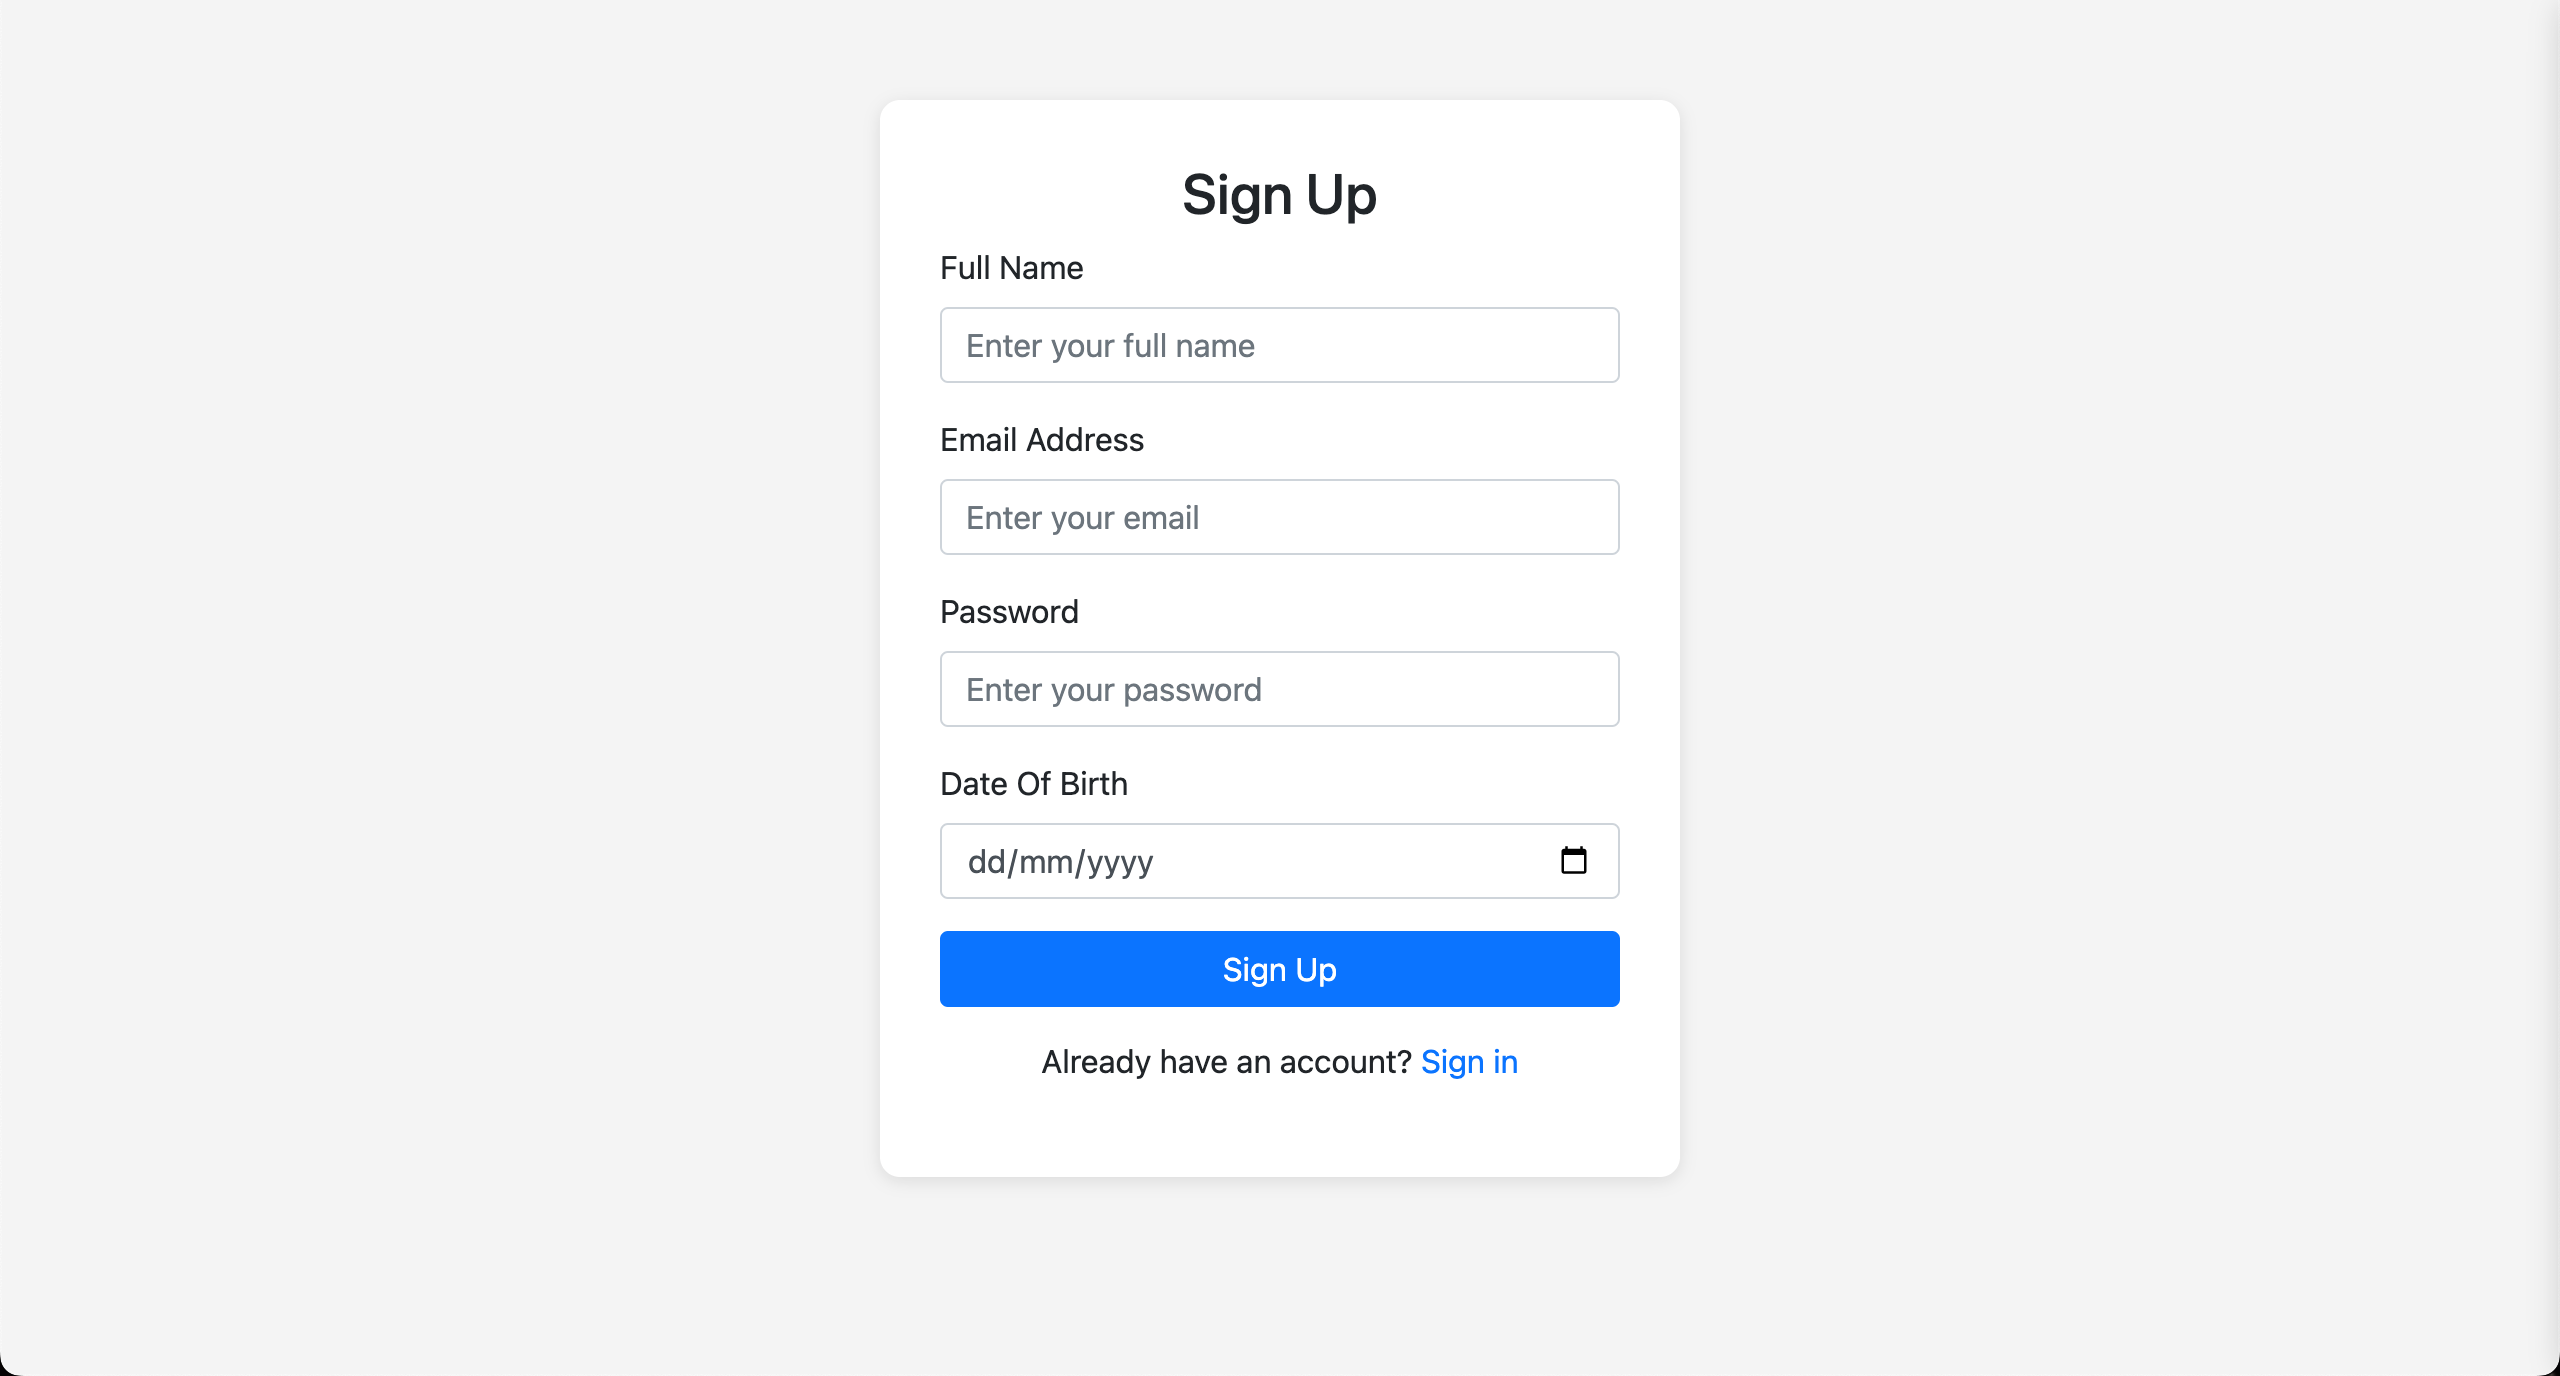
\includegraphics[width=\textwidth]{signup.png}
    \caption{User Registration Form}
    \label{fig:signup}
\end{figure}

Once registered and logged in, users can share their experiences by accessing the "Share Your Experience" form, as shown in Figure \ref{fig:share}. This form allows users to input the location of their experience and provide a detailed description. Additionally, users can upload images or videos to enhance their posts, making the shared experiences more vivid and engaging for other users.

\begin{figure}[H]
    \centering
    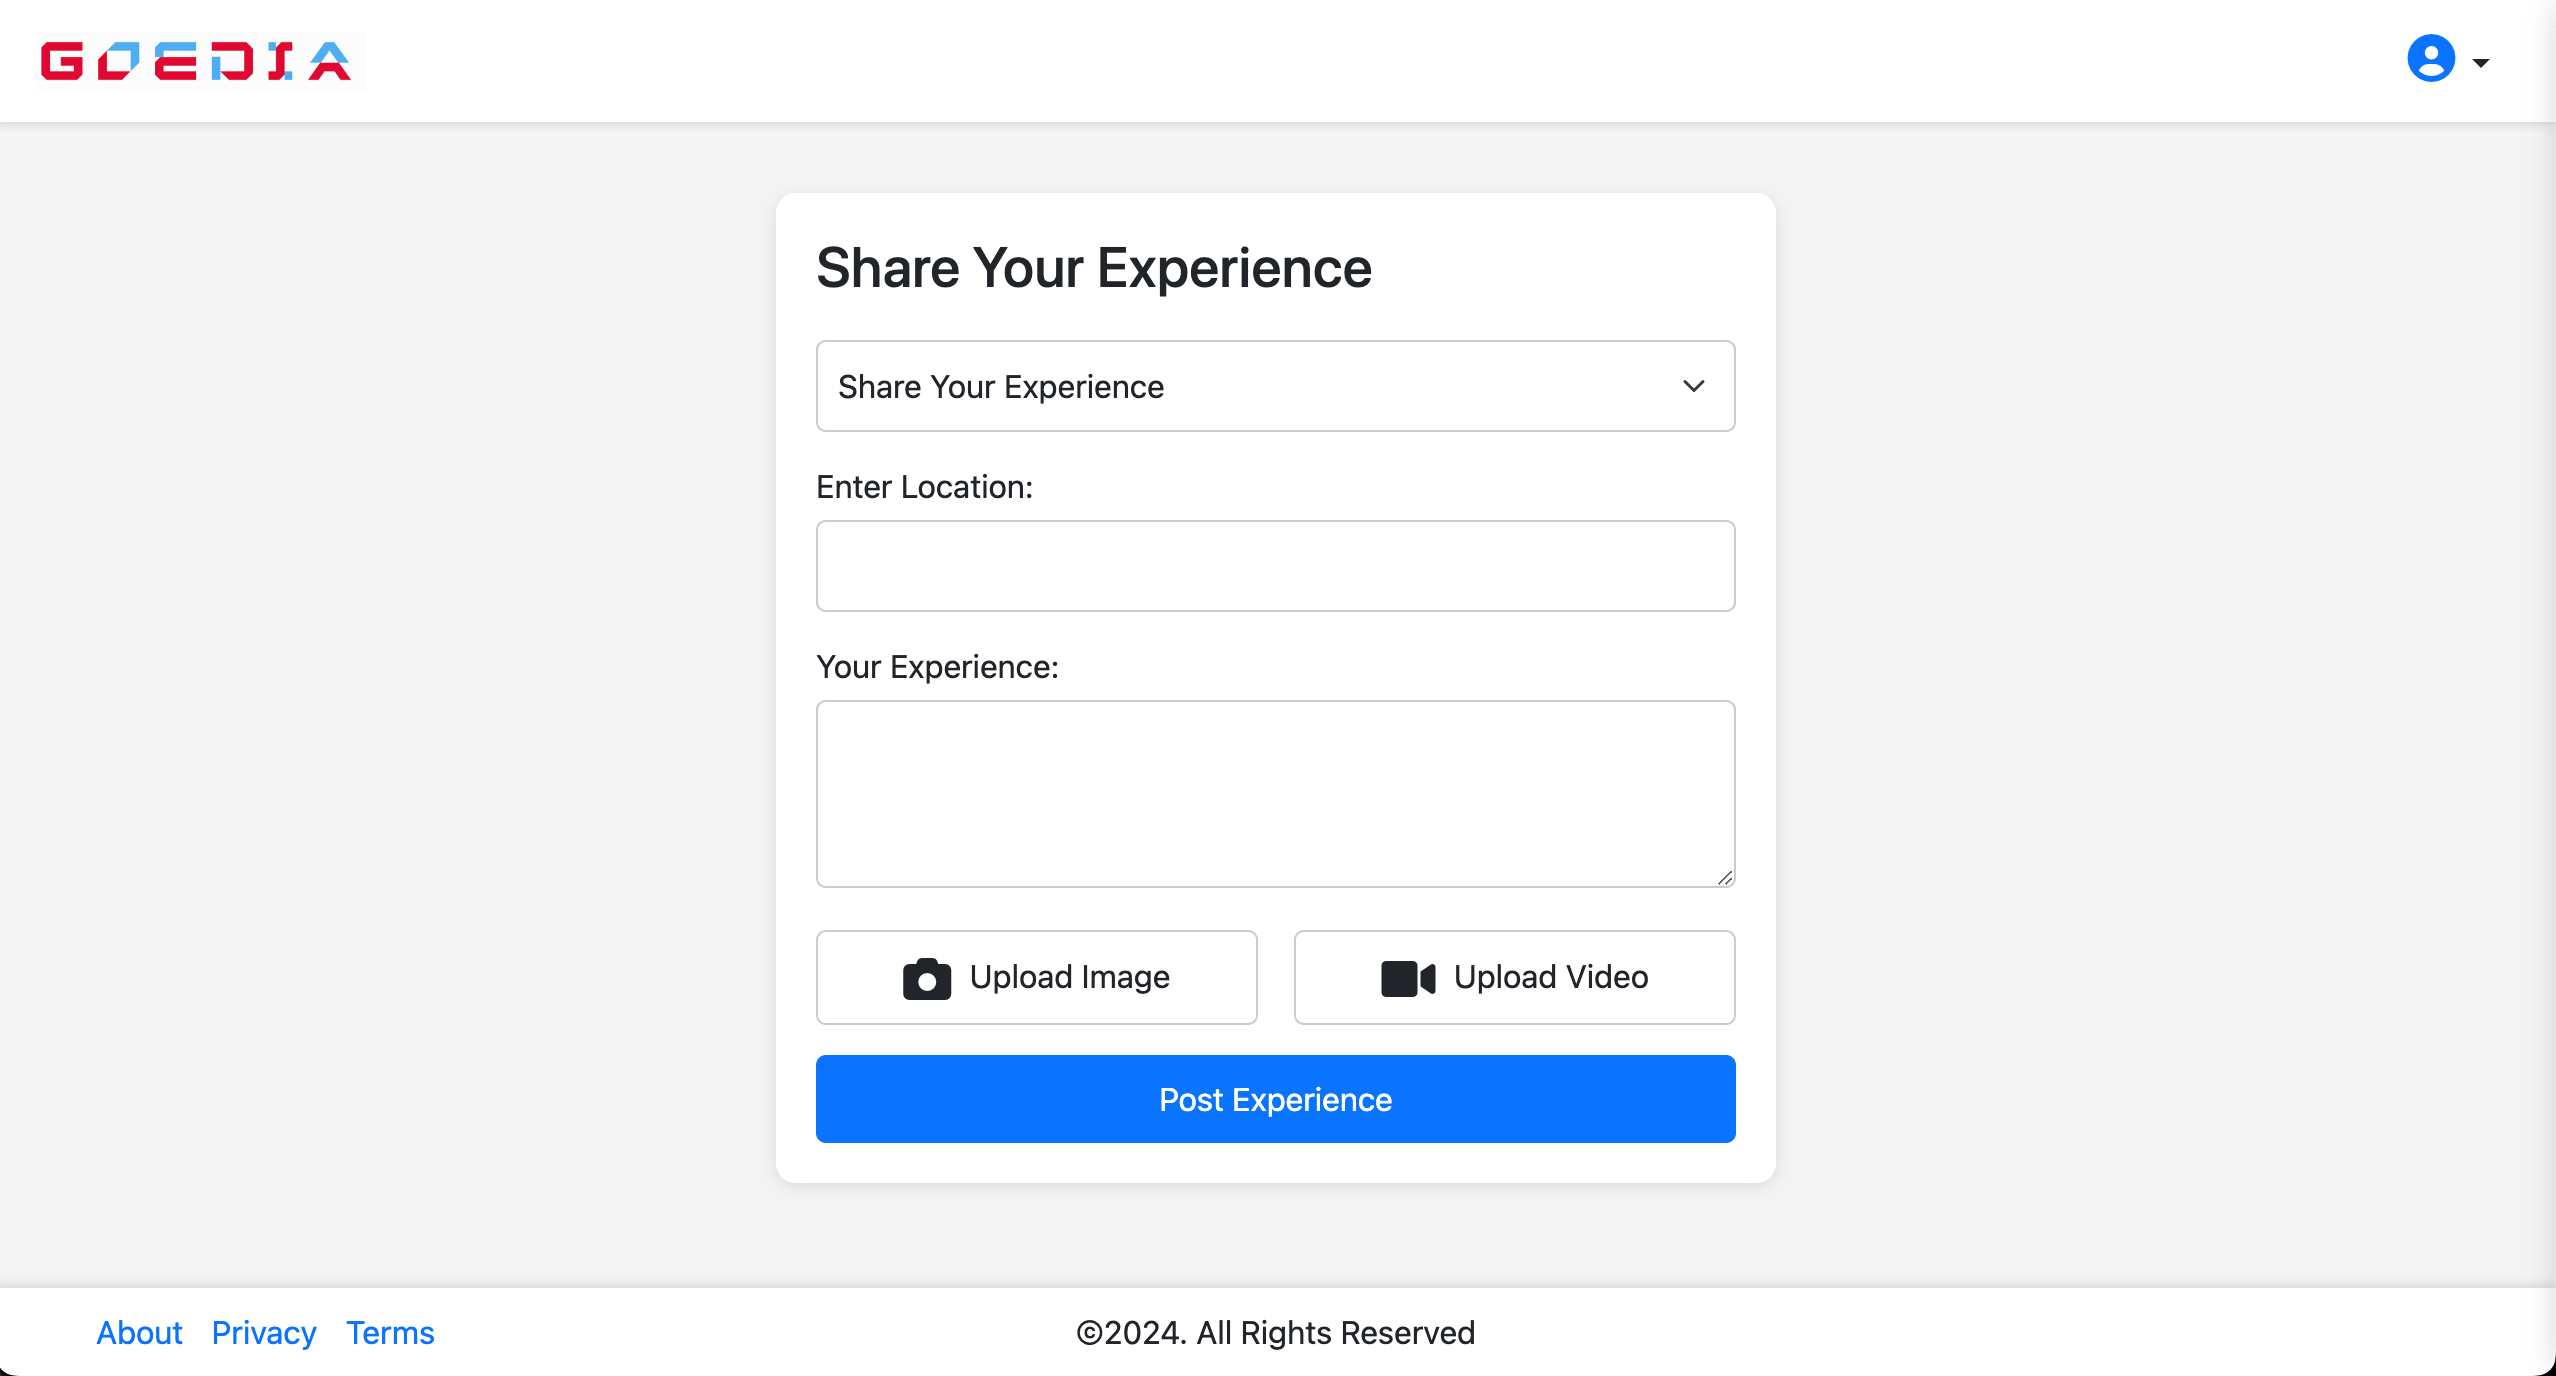
\includegraphics[width=\textwidth]{share.png}
    \caption{Share Your Experience Form}
    \label{fig:share}
\end{figure}

Each user has a personal account page where they can view their profile information and their posts. Figure \ref{fig:useraccount} illustrates this account page, which displays the user's email, date of birth, and a list of their posts. This page serves as a personal dashboard for users to manage their contributions to the platform.

\begin{figure}[H]
    \centering
    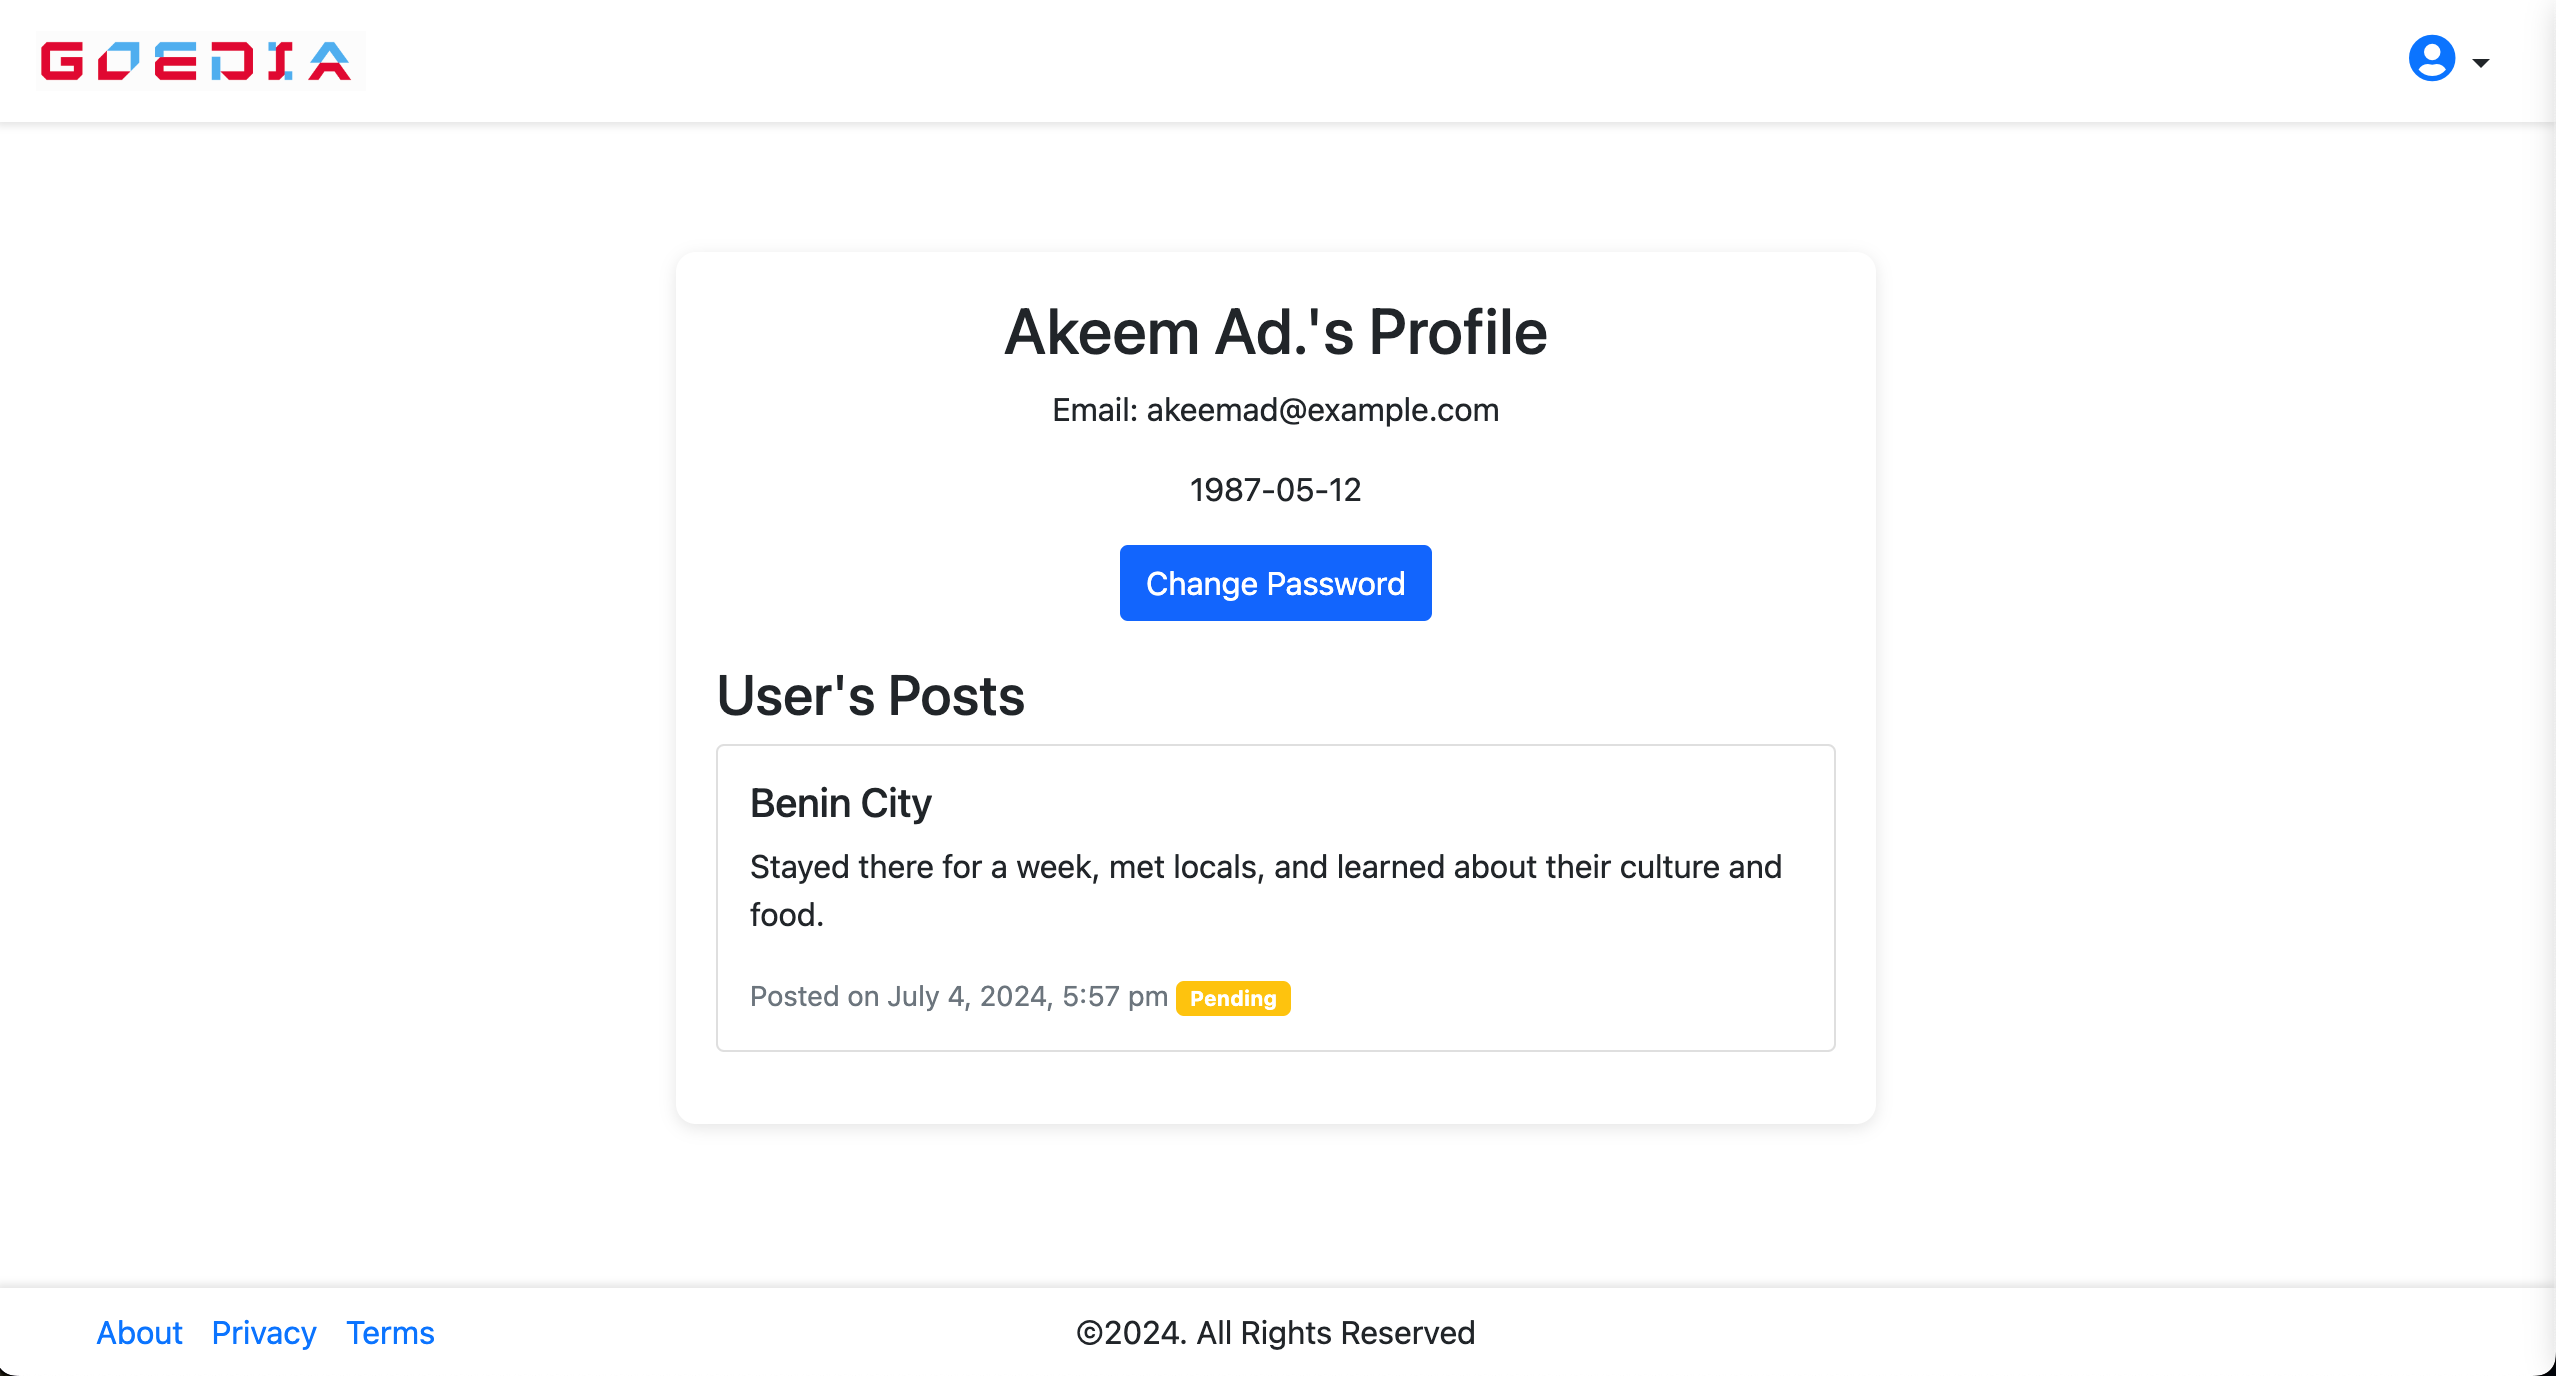
\includegraphics[width=\textwidth]{useraccount.png}
    \caption{User Account Page}
    \label{fig:useraccount}
\end{figure}

The experience feed, shown in Figure \ref{fig:userfeed}, is a central feature of the application, where users can browse through posts shared by others. This feed is continuously updated with new experiences, enabling users to discover new places and insights from the community. The layout is designed to be visually appealing and easy to navigate, ensuring a pleasant browsing experience.

\begin{figure}[H]
    \centering
    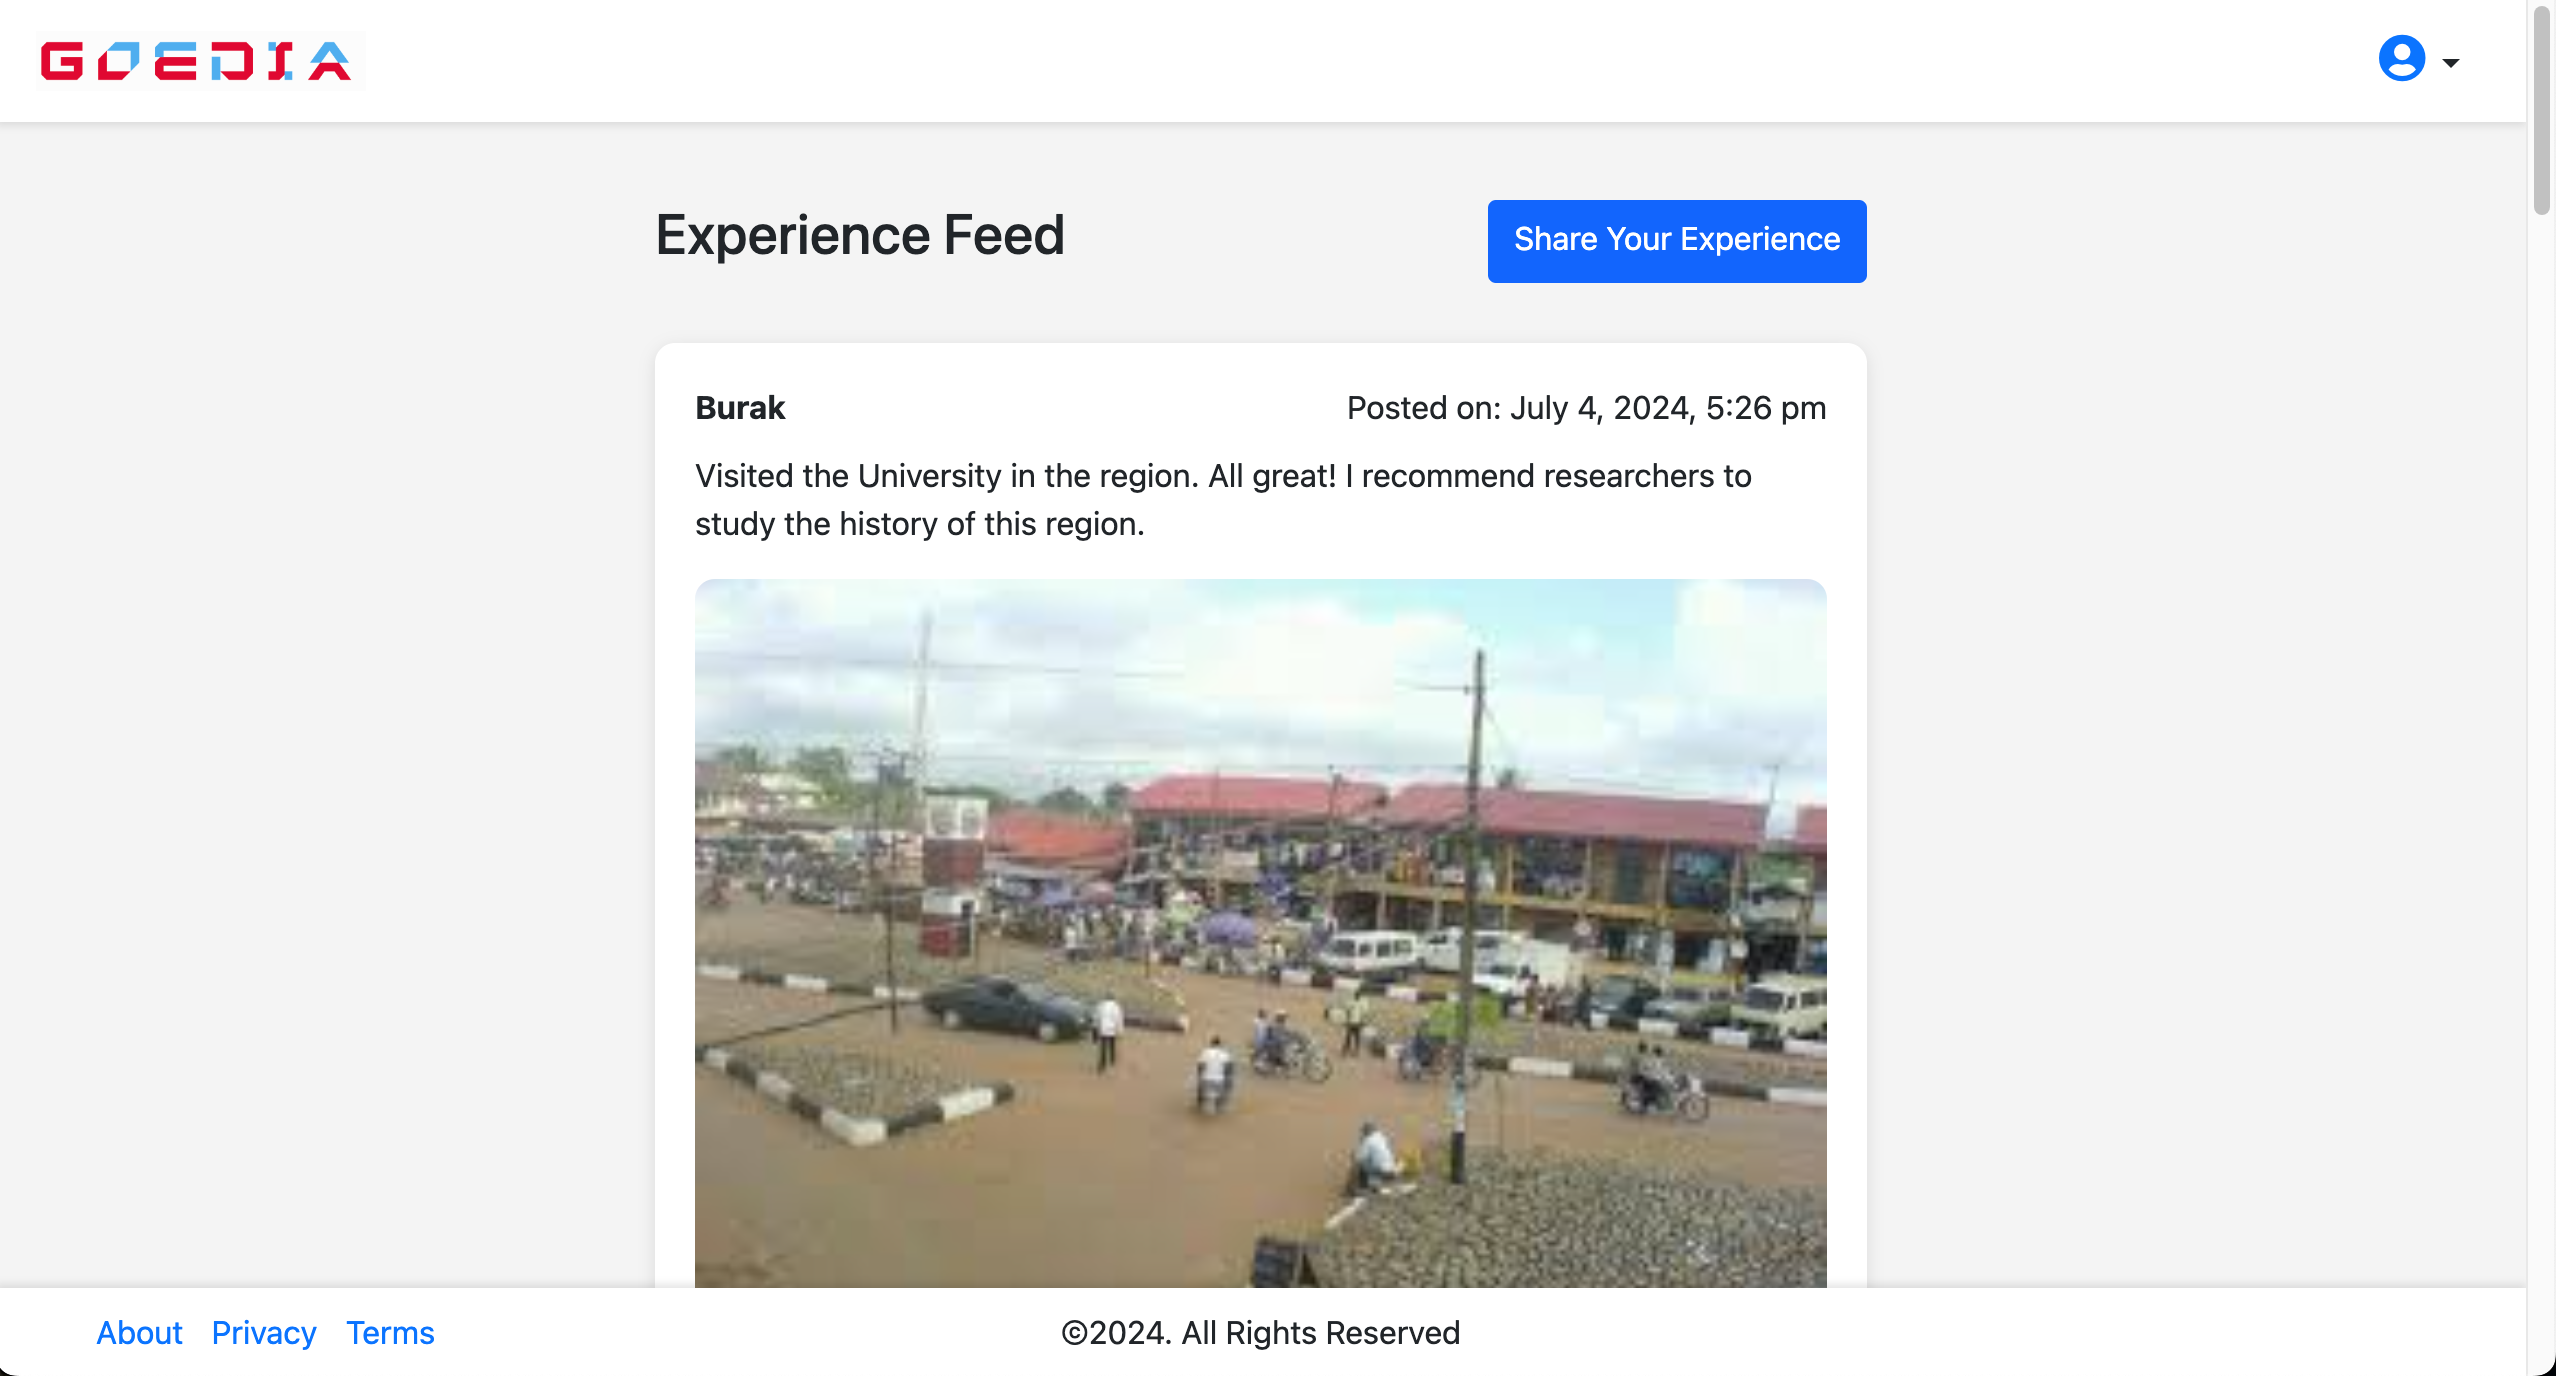
\includegraphics[width=\textwidth]{userfeed.png}
    \caption{Experience Feed}
    \label{fig:userfeed}
\end{figure}

Figure \ref{fig:placedetails} shows the place details page that users are directed to after a search. This page provides a map of the location, detailed descriptions, and user reviews. The integration of a map enhances the usability of the platform by helping users visualize the location and its surroundings.

\begin{figure}[H]
    \centering
    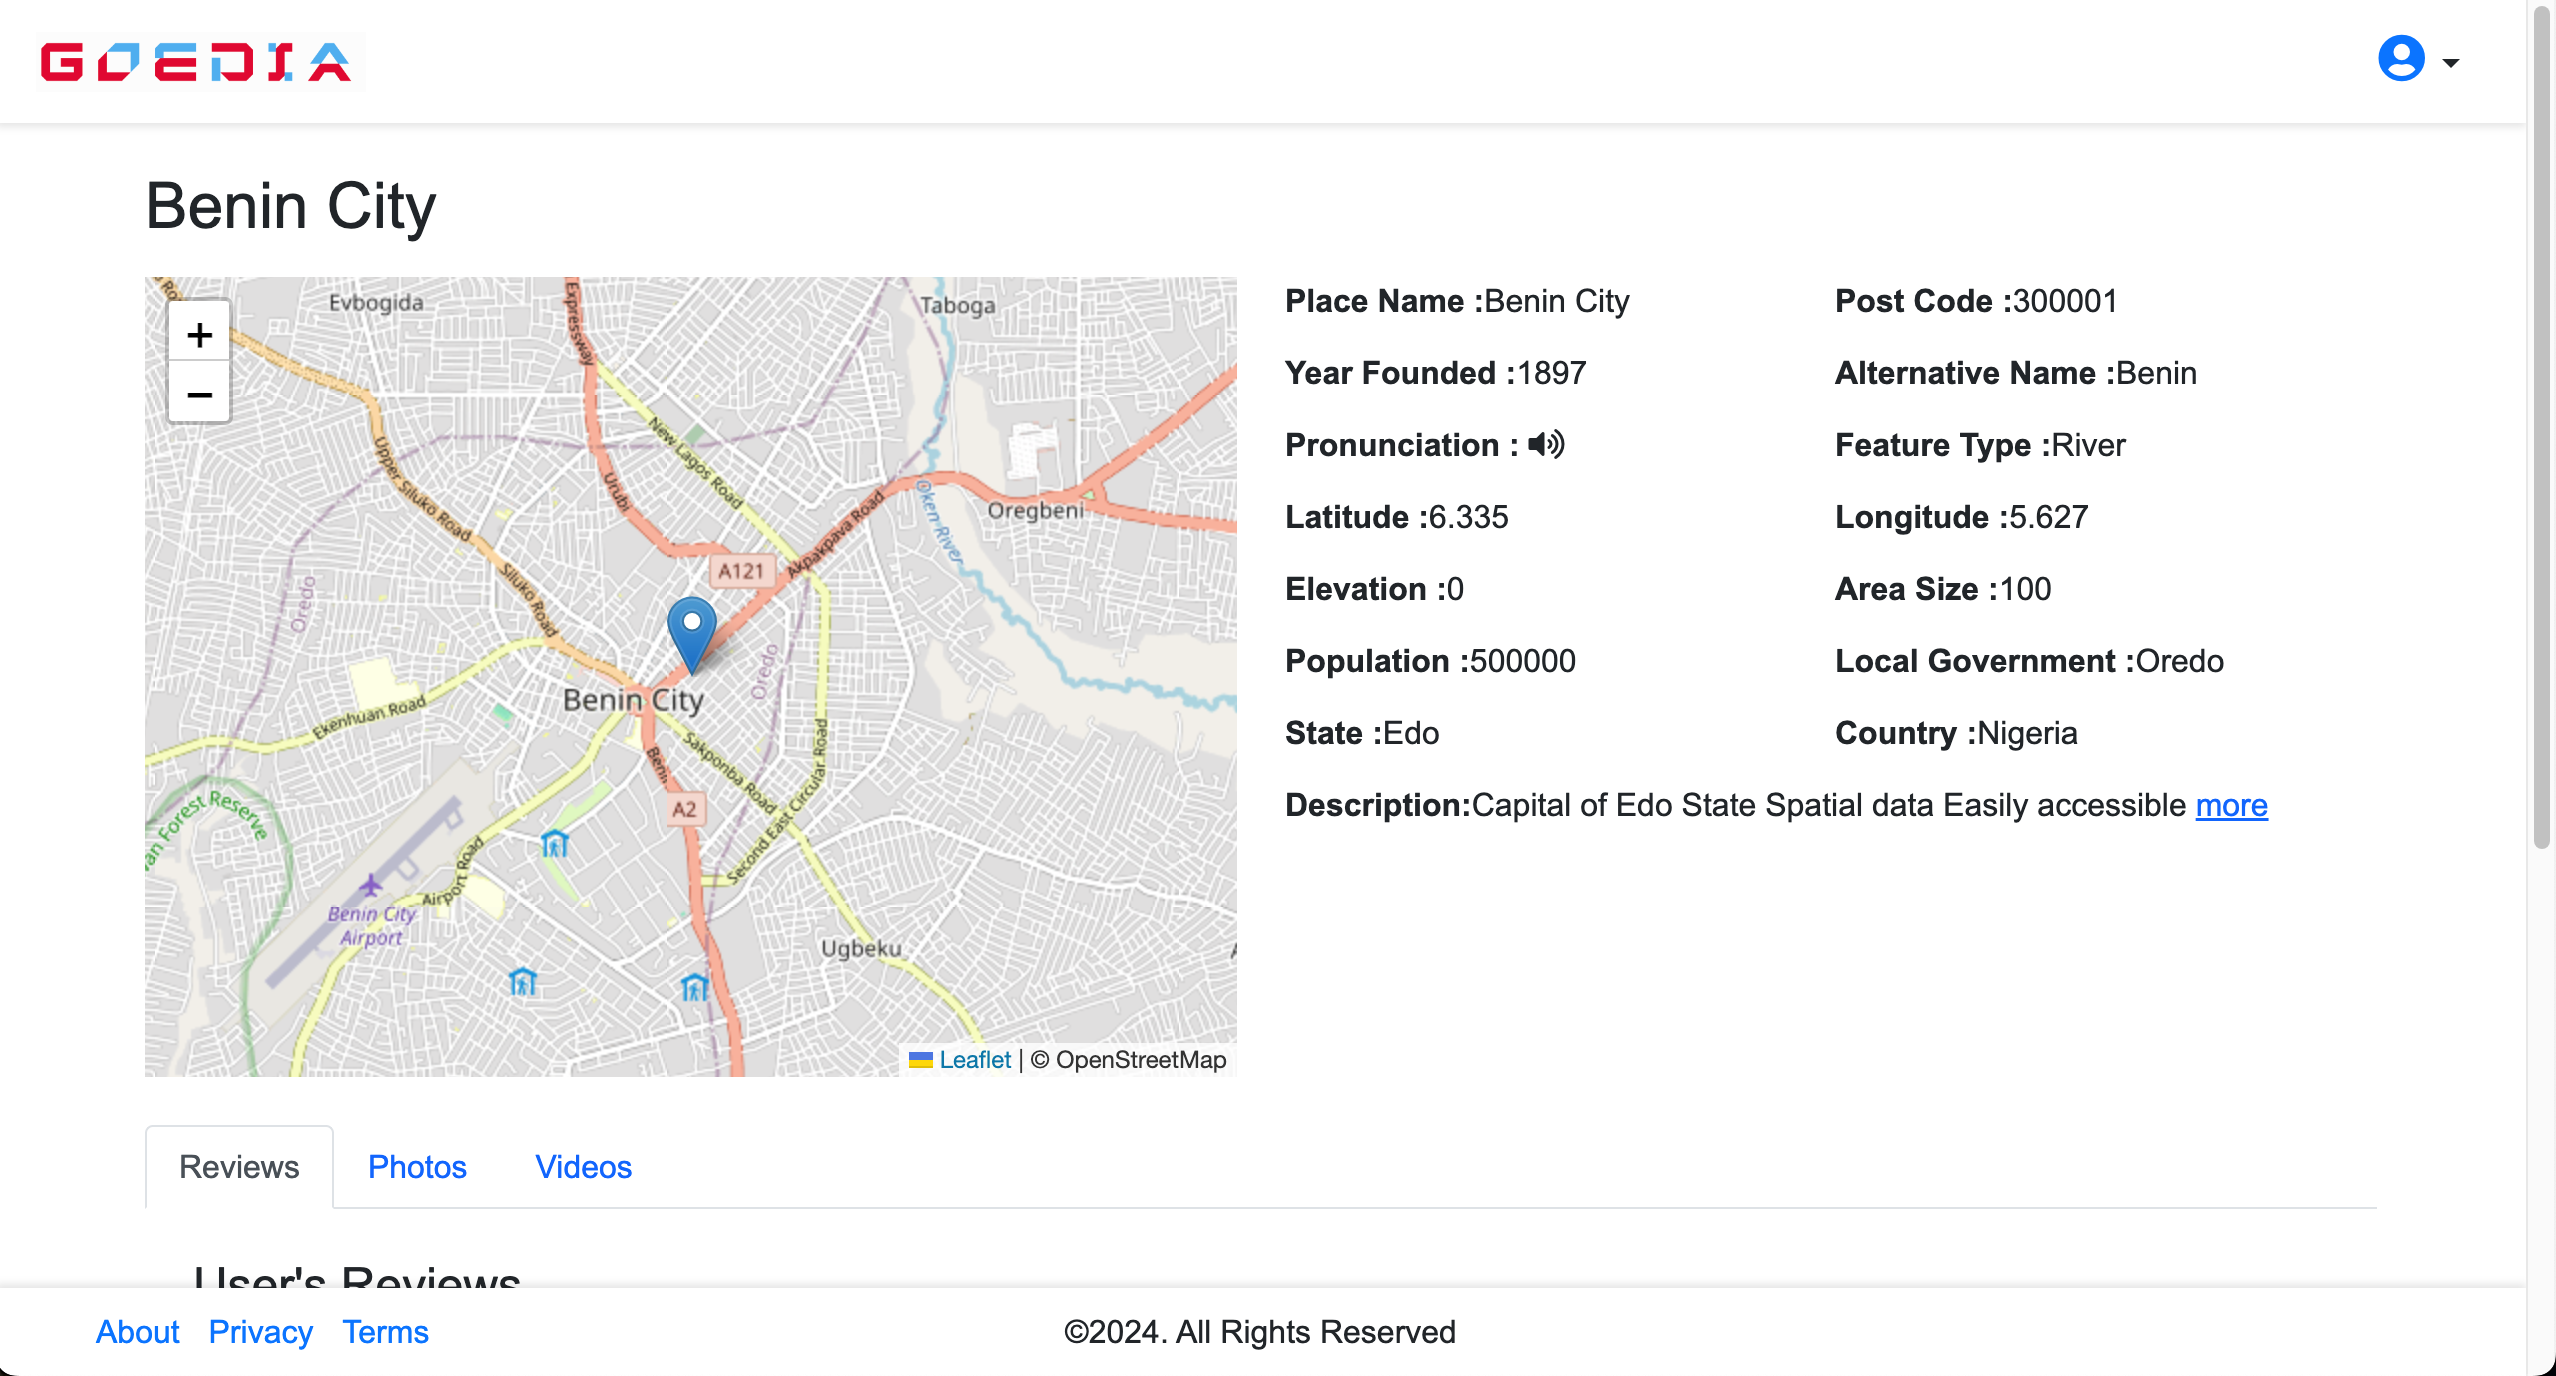
\includegraphics[width=\textwidth]{placedetails.png}
    \caption{Place Details Page}
    \label{fig:placedetails}
\end{figure}

Administrators of the platform have access to a comprehensive dashboard, as shown in Figure \ref{fig:admindashboard}. This dashboard presents various statistics in graphical formats, such as bar charts and pie charts. These visualizations help administrators monitor the platform's activity, including the member with the highest number of posts and the most visited places.

\begin{figure}[H]
    \centering
    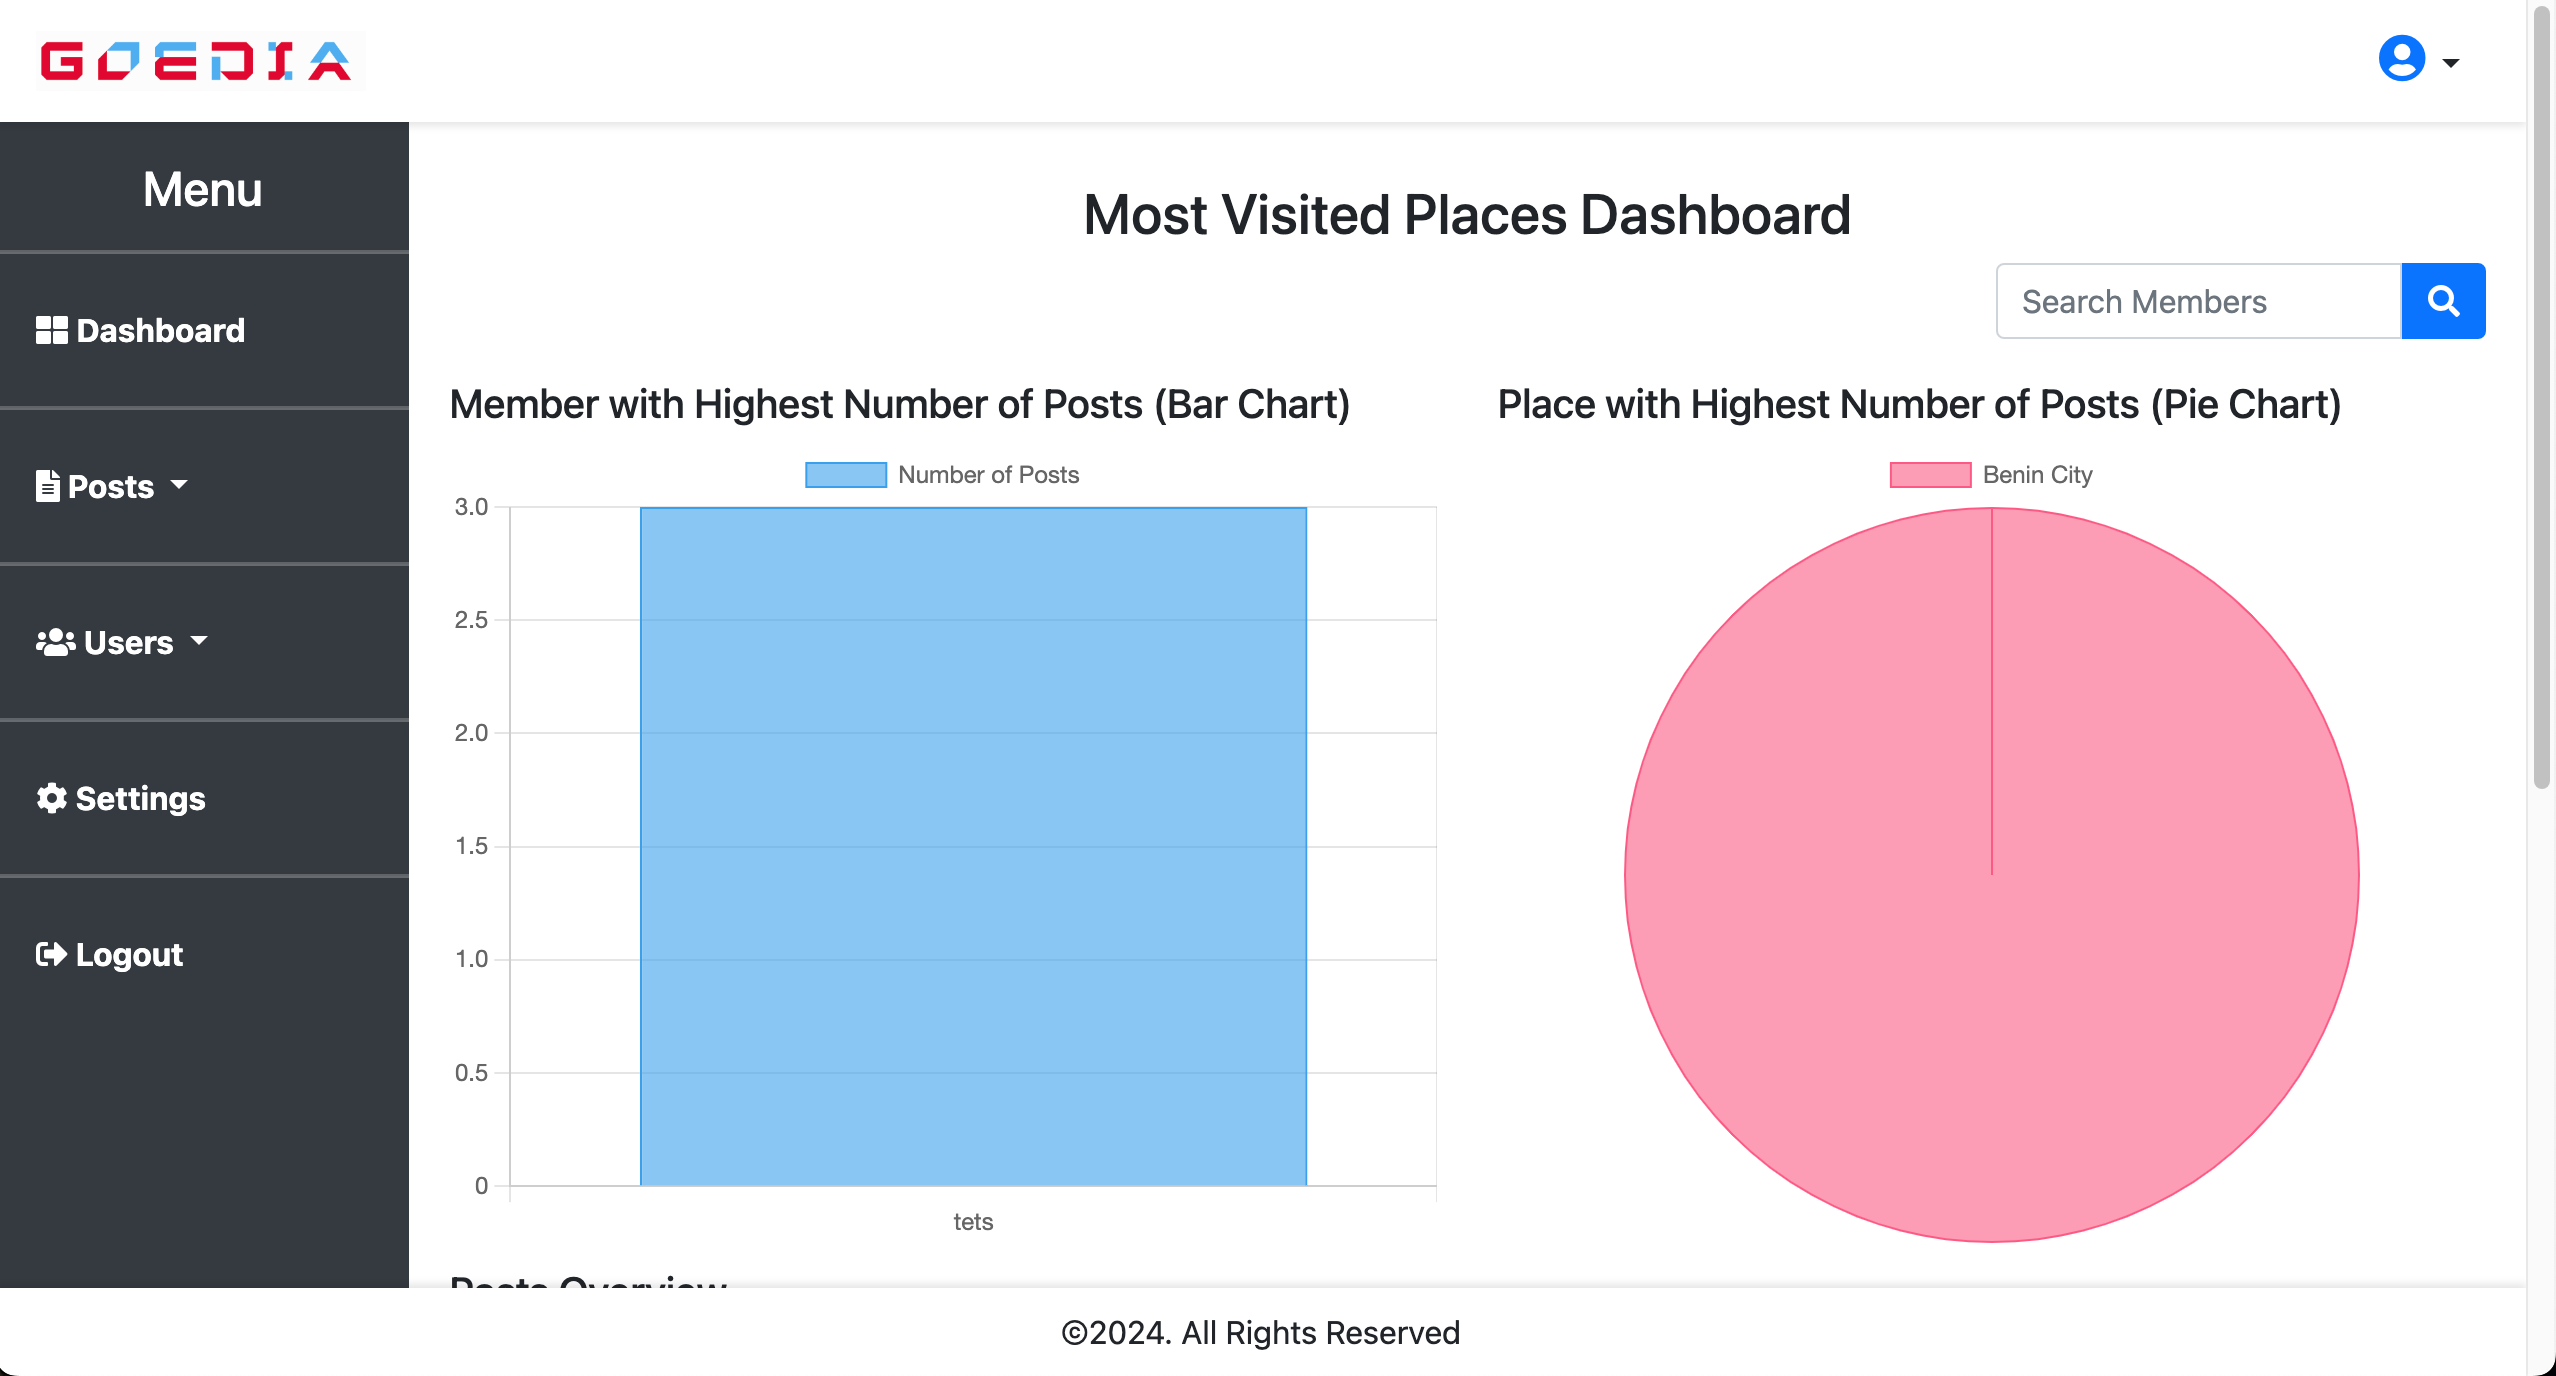
\includegraphics[width=\textwidth]{admindashboard.png}
    \caption{Admin Dashboard with Statistics}
    \label{fig:admindashboard}
\end{figure}

Administrators are also responsible for approving or rejecting user posts. Figure \ref{fig:approveposts} displays the user posts management page, where administrators can view all submitted posts and their current status. This page allows admins to ensure that only appropriate content is published on the platform.

\begin{figure}[H]
    \centering
    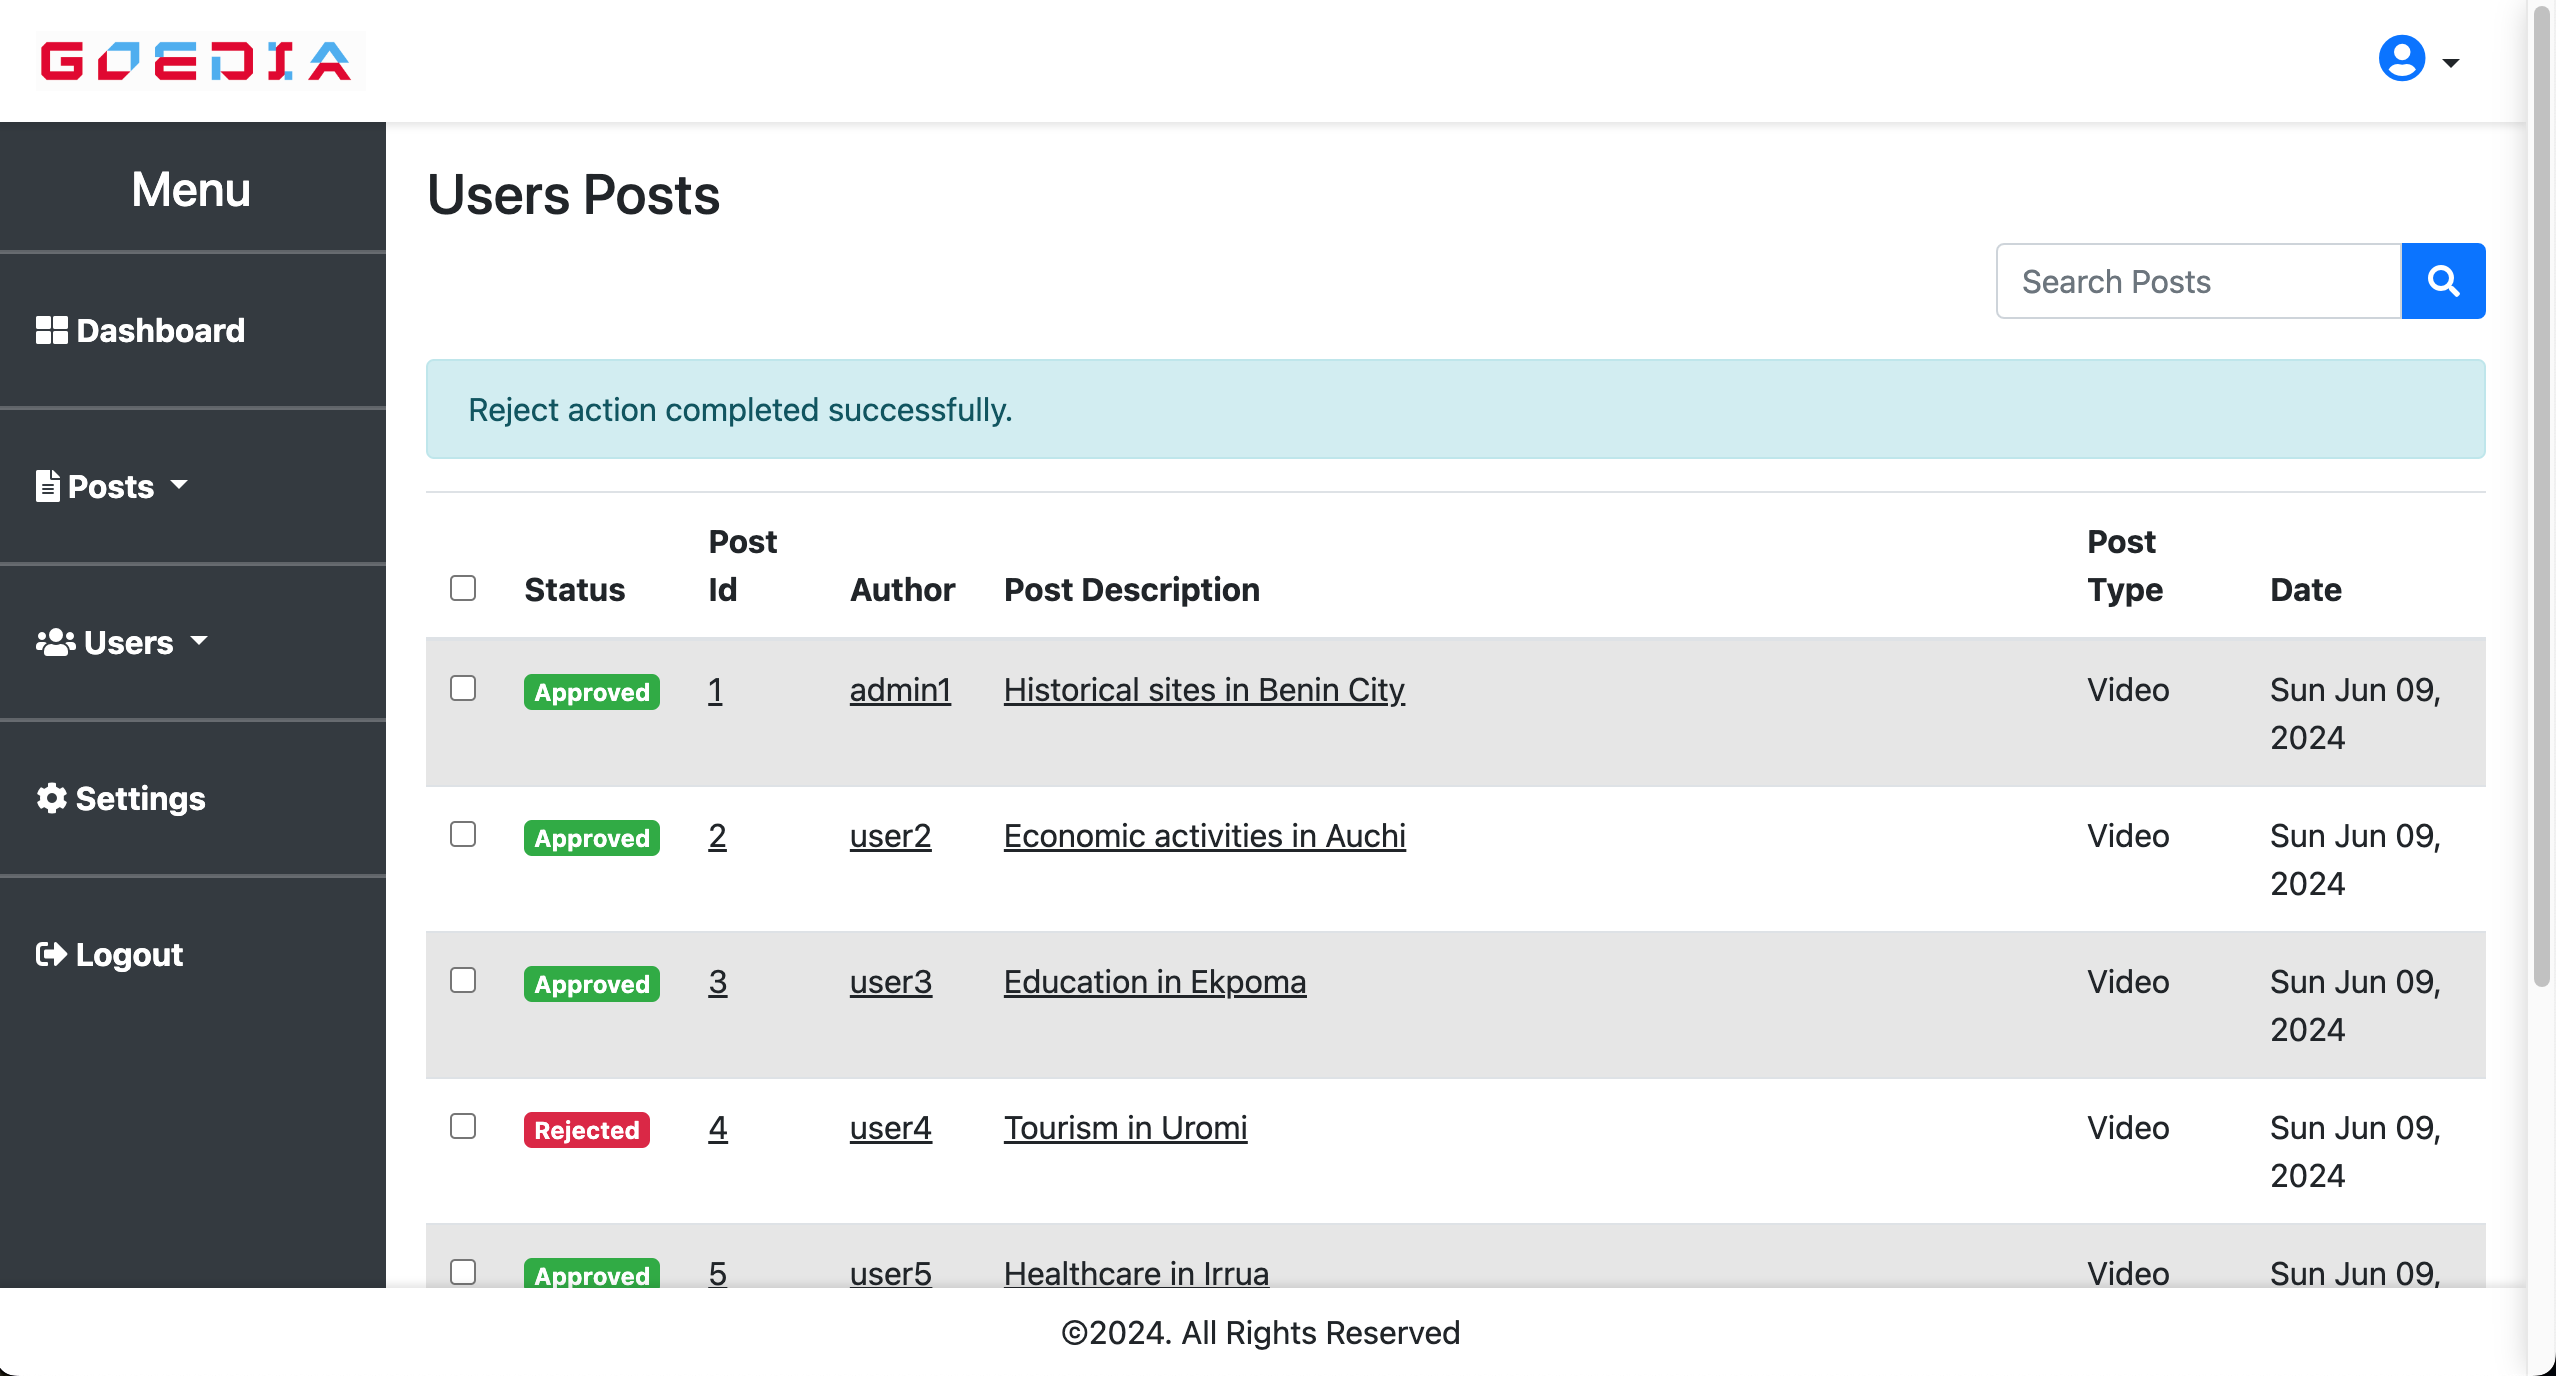
\includegraphics[width=\textwidth]{approveposts.png}
    \caption{Admin Page for Approving or Rejecting Posts}
    \label{fig:approveposts}
\end{figure}

Furthermore, administrators can manage user statuses through the admin view of user statuses, depicted in Figure \ref{fig:seeusersstatus}. This functionality allows admins to track active members, their post counts, and their last seen activity, thereby maintaining an organized and well-functioning user base.

\begin{figure}[H]
    \centering
    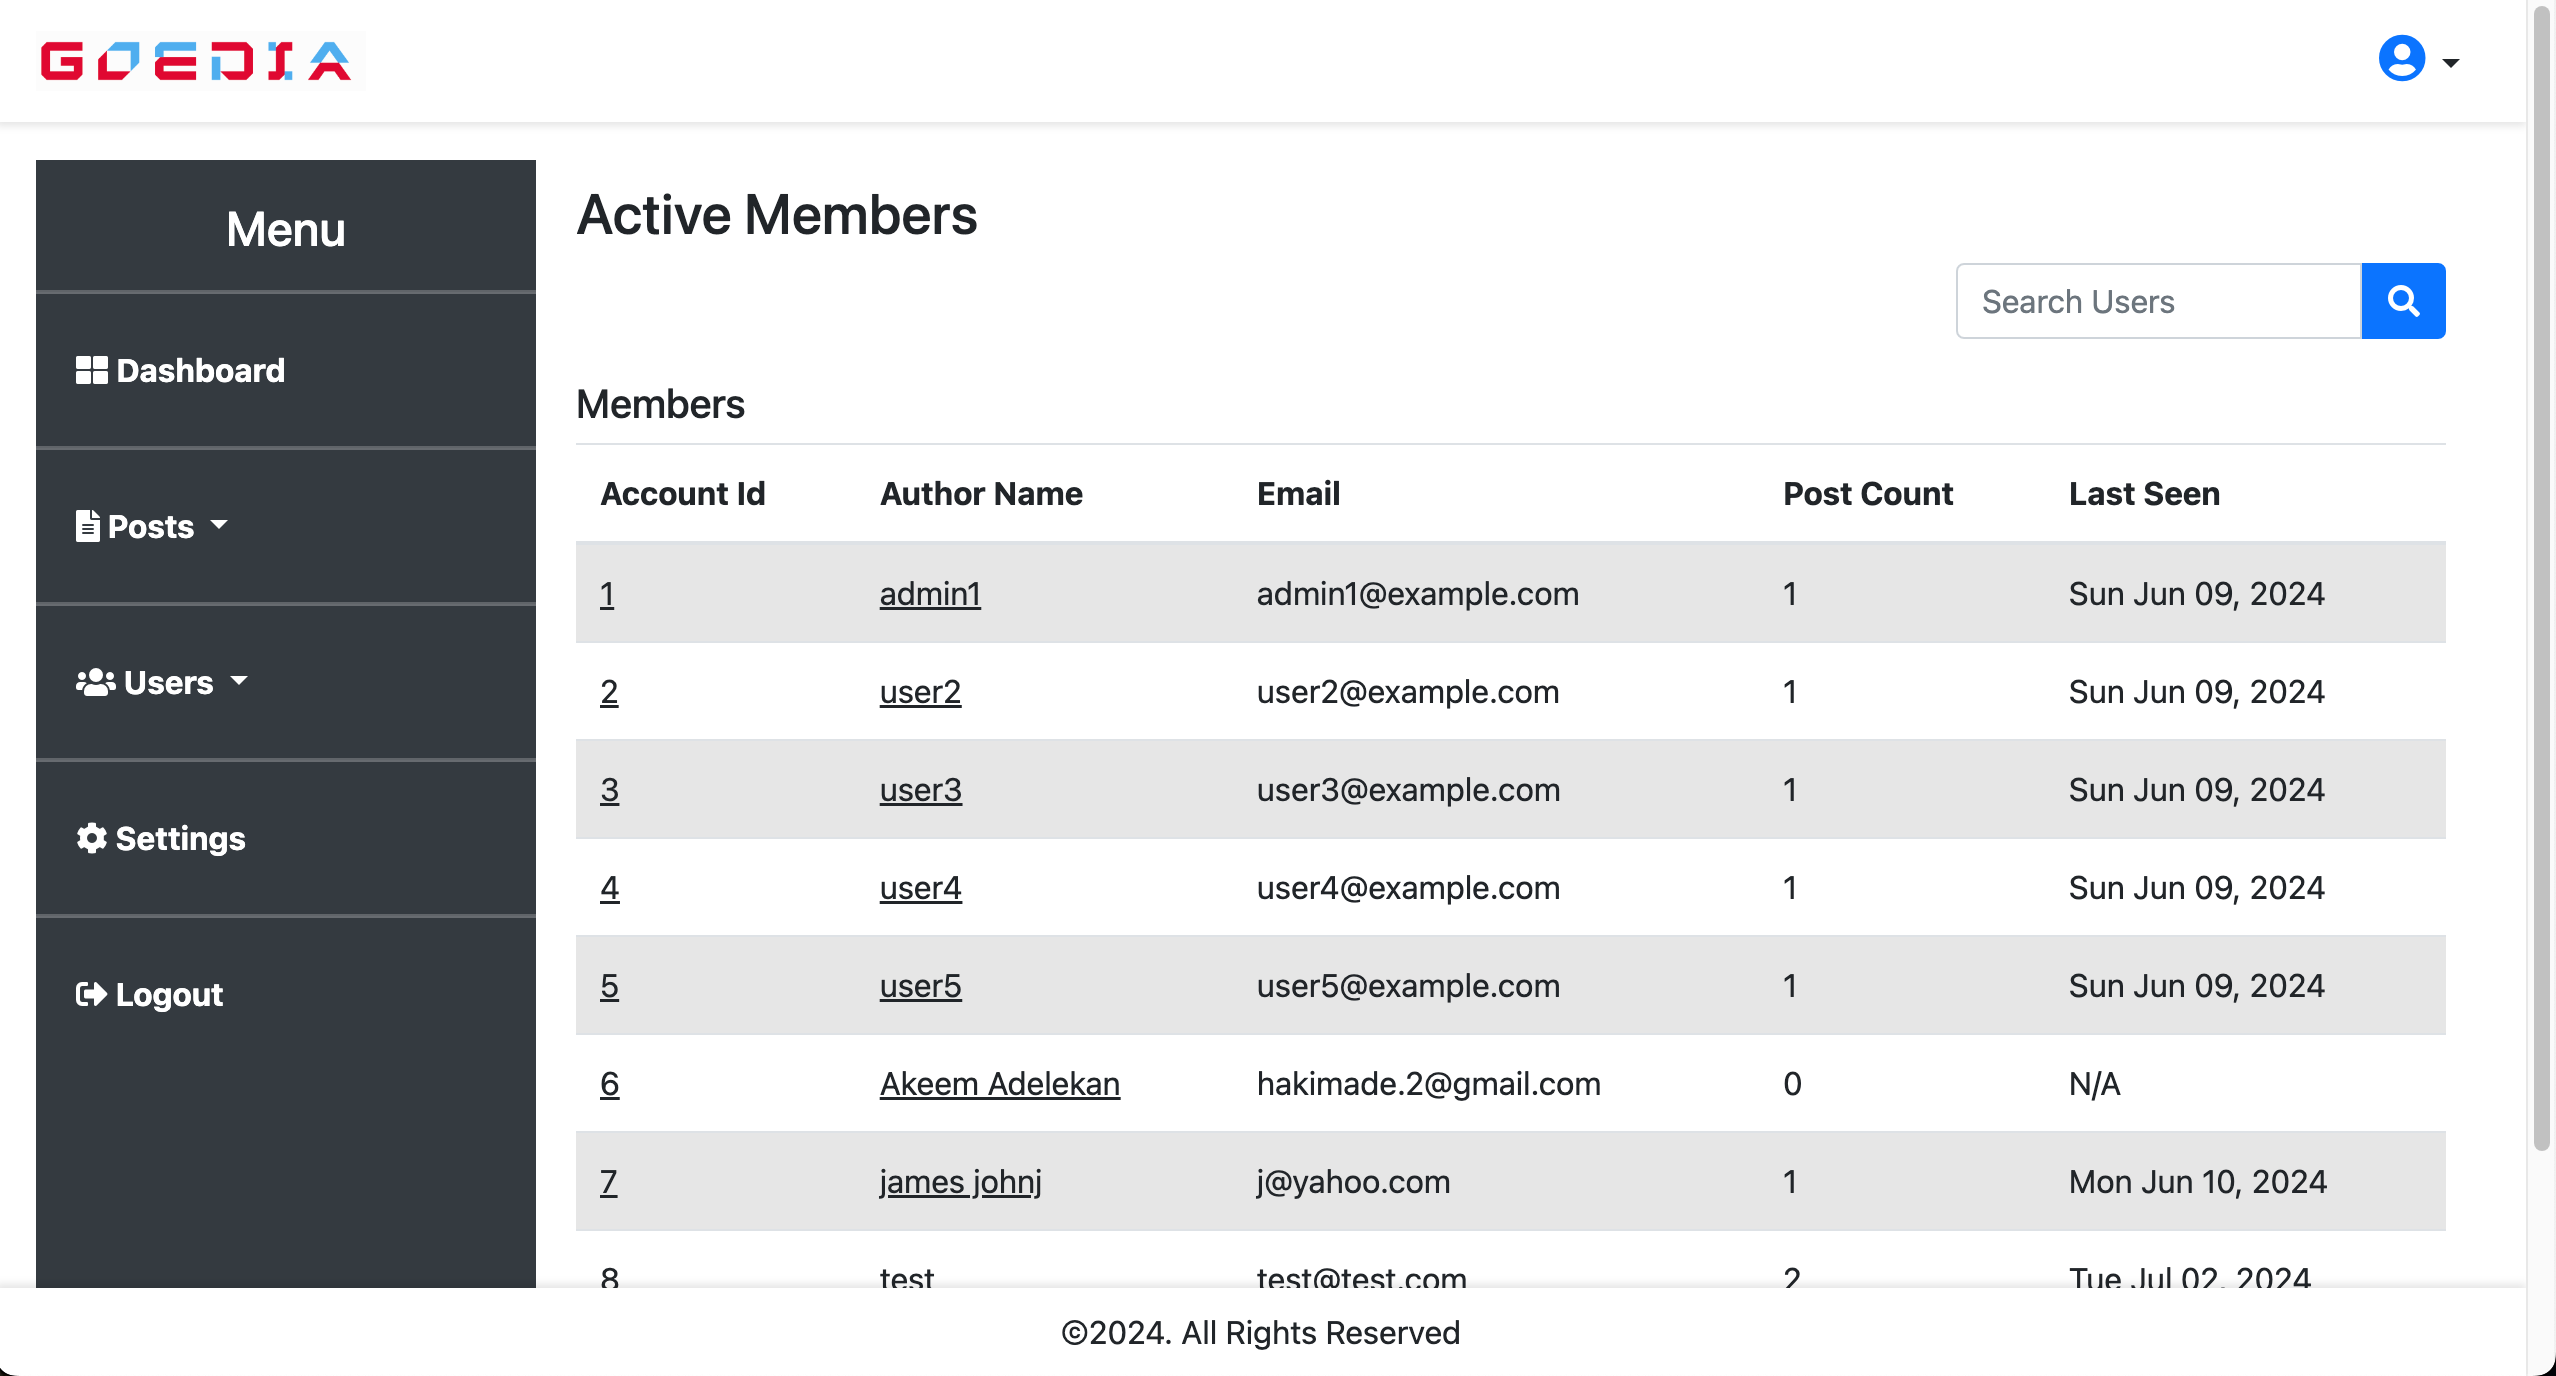
\includegraphics[width=\textwidth]{seeusersstatus.png}
    \caption{Admin View of User Statuses}
    \label{fig:seeusersstatus}
\end{figure}

Lastly, the platform enables administrators to add new place details through a dedicated form, as illustrated in Figure \ref{fig:addnewplace}. This form allows admins to input essential information about new locations, such as the place name, postcode, year founded, and a description. Adding new places helps in expanding the platform's database and providing users with more options to explore.

\begin{figure}[H]
    \centering
    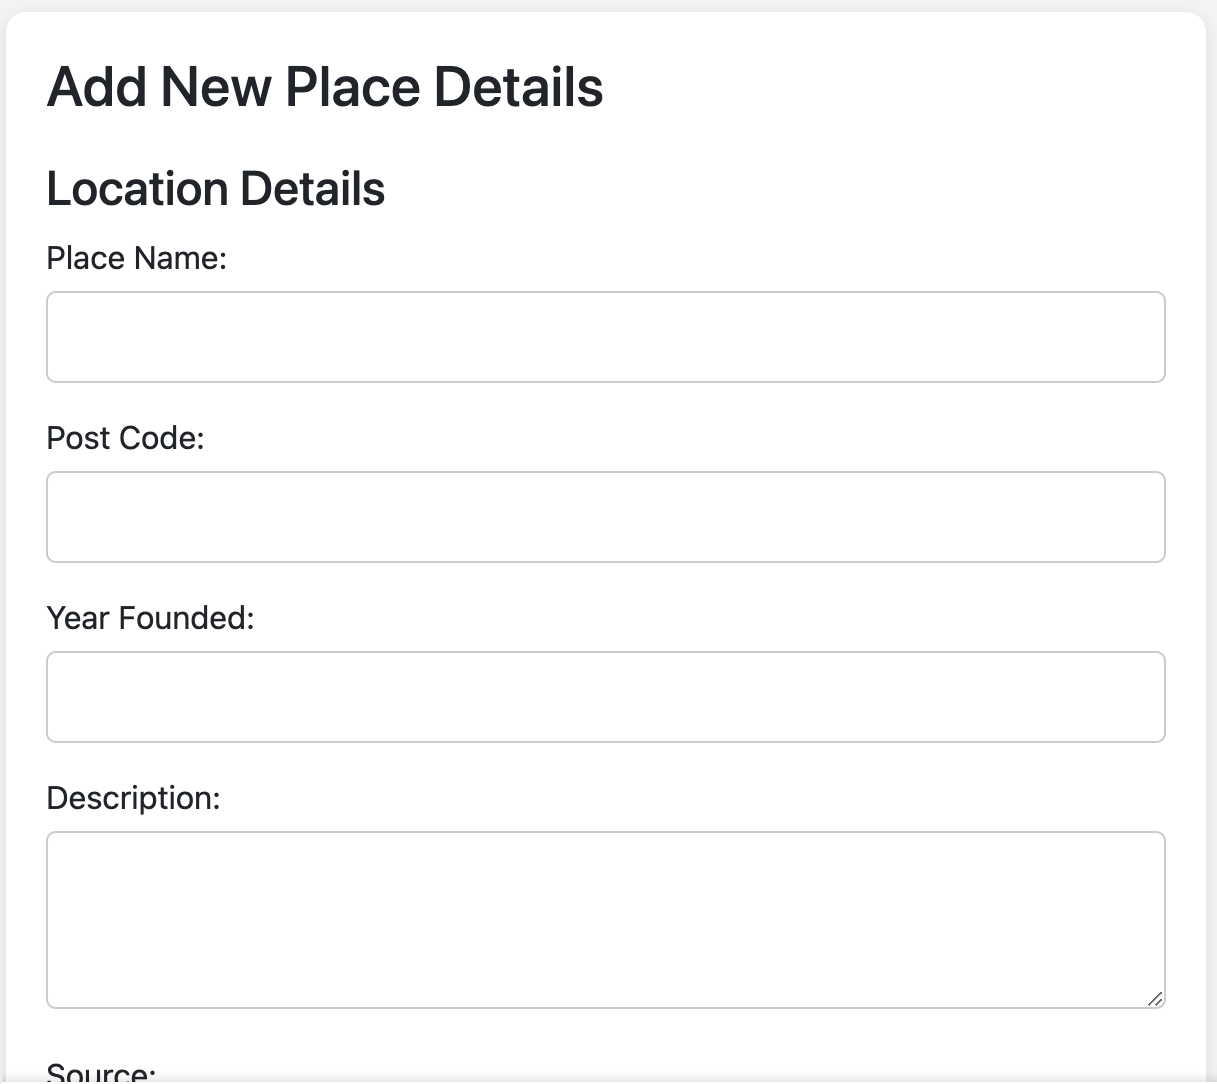
\includegraphics[width=\textwidth]{addnewplace.png}
    \caption{Form to Add New Place Details}
    \label{fig:addnewplace}
\end{figure}

These screenshots collectively demonstrate the comprehensive capabilities and functionalities of our application. They highlight how users can interact with the platform to share and discover experiences, while administrators can manage content and users effectively. This chapter serves as a practical guide to understanding the user experience and the administrative controls within the application.